\documentclass[14pt]{mmcs-article}
\usepackage[russian]{babel}
\usepackage{amsmath, amsthm, amsfonts, amssymb}

\graphicspath{{images/}}

\begin{document}

\section*{Введение}

\textbf{Определение 1.}

%Вводим определение пути, вводим первую, последнюю вершины пути (словами, можно подсмотреть в книжке Ерусалимского). Тут же определем циклы.

\textsl{Двудольным графом} будем называть пару $\langle V,E \rangle$, такую, что:

\begin{itemize}
    \item $V = A \cup B$ и $A \cap B = \emptyset$ ;
    \item $e = (a, b), a \in A, b \in B \forall e \in E$;
\end{itemize}

Где $V$ ~--- множество вершин, разбитое на два непересекающихся подмножества $A$ и $B$.
$E$ ~--- множество дуг. Дуга ~--- это упорядоченная пара вершин, называемых инцидентными этой дуге.

\textbf{Определение 2.}

Пусть $G$ ~--- граф $G = \langle A \cup B, E \rangle$.
Упорядоченную последовательность дуг $\psi = (e_1, ..., e_d)$ будем называть путём, если $\forall i = 2..d$ у вершин $e_{i-1}$ и $e_i$ есть инцидентная вершина.

\textbf{Определение 3.}

Первой вершиной пути $\psi = (e_1, ..., e_d)$ будем называть вершину, инцидентную дуге $e_1$, но не инцидентную вершине $e_2$.

Последней вершиной пути $\psi = (e_1, ..., e_d)$ будем называть вершину, инцидентную дуге $e_d$, но не инцидентную вершине $e_{d-1}$.

\textbf{Определение 4.}

Циклом будем называть путь, у которого совпадают первая и последняя вершины.

\textbf{Определение 5.}

\textsl{Обхватом графа} называют длину его минимального цикла.

\textbf{Замечание 1.}

Отметим, что обхват любого двудольного графа является чётным числом, большим, чем два.

\textbf{Замечание 2.}

Известно, что на практике для кодирования эффективнее использовать графы с большим обхватом.

\pagebreak
\section*{Метаграфы}

\textbf{Определение 3.}

\textsl{Метаграфом} будем называть тройку $\langle A \cup B,E,w \rangle$, такую, что:

\begin{itemize}
    \item $\langle A \cup B,E \rangle$ ~--- двудольный граф;
    \item $w: E \rightarrow \mathbb{Z}$ ~--- отображение задающее веса дуг.
\end{itemize}

На (рис. \ref{image:2}) представлен пример метаграфа с тремя вершинами и четырьмя дугами.

\begin{figure}[H]
    \centering
    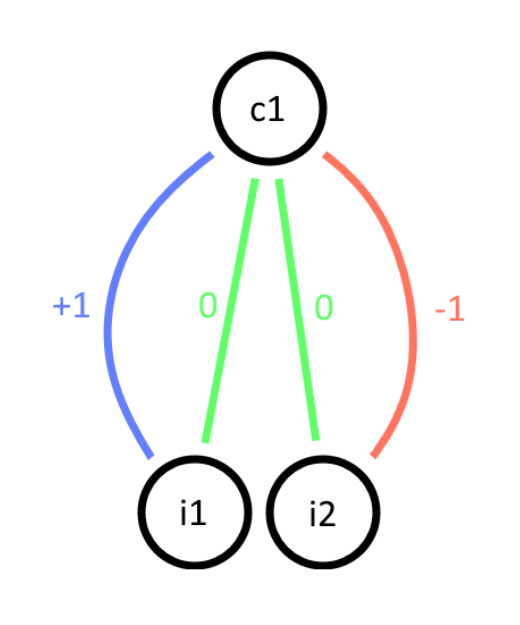
\includegraphics[scale=0.4]{Fig_2.png}
    \caption{ Метаграф с весами дуг +1, 0, 0, -1.. }
    \label{image:2}
\end{figure}

Пусть $G$ ~--- метаграф, $G = \langle V, E, w \rangle$, и задано число $r \in \mathbb{N}$. Построим двудольный граф $G^{(r)} = \langle V', E' \rangle$ по следующим правилам:

% Введём обозначение для множества вершин или дуг, порождаемых из одной вершины или дуги в процессе расширения метаграфа:



\begin{itemize}
    \item Каждой вершине $v \in V$ поставим в соответствие множество вершин 
    \[
        T^{(r)}_v = \{ v^{(i)} | v \in V \}
    \]
    Будем говорить, что вершины из этого множества соответствуют вершине $v$ и наоборот;
    
    \item Каждой дуге $e \in E$ (для определённости будем считать,что $e = (a, b)$) ставится в соответстие множество дуг 
    \[
        T^{(r)}_e = \{ (a^{(j)}, b^{(j + w(e) (mod\ r))} | j = 1..r \}
    \]
    Будем говорить, что дуги из этого множества соответствуют дуге $e$ и наоборот;
    \item Положим 
    \[
        V' = \bigcup_{v \in V} T^{(r)}_v; E' = \bigcup_{e \in E} T^{(r)}_e.
    \]
\end{itemize}

\textbf{Определение 4.}

Граф $G^{(r)}$, построенный в ходе работы Алгоритма 1. будем называть расширением метаграфа $G$ в $r$ раз.

На (рис. \ref{image:3}) изображён граф, полученный расширением метаграфа из (рис. \ref{image:2}) в 4 раза.

\begin{figure}[H]
    \centering
    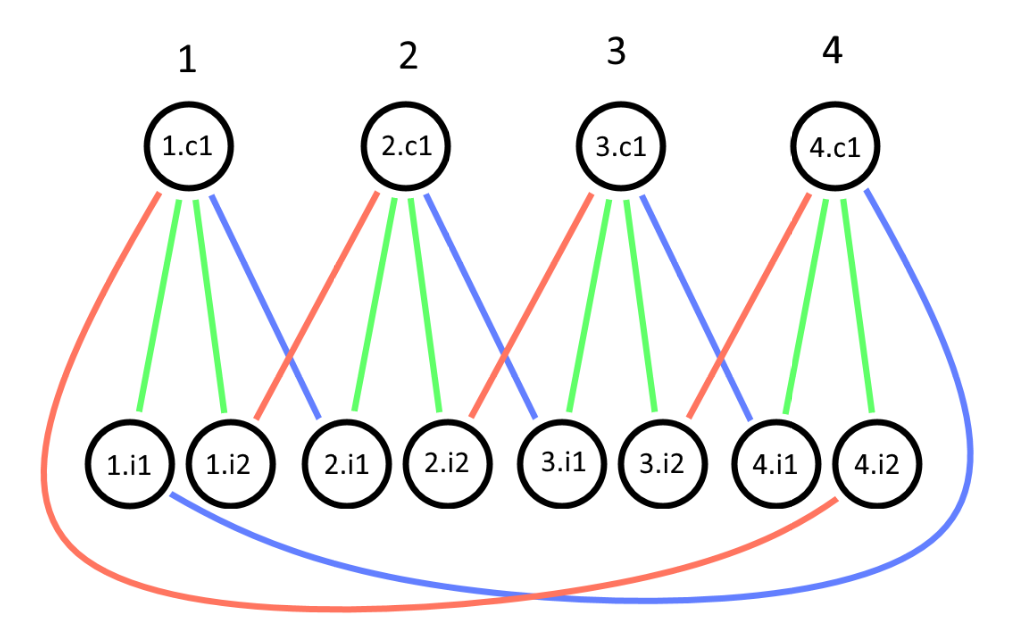
\includegraphics[scale=0.4]{Fig_1.png}
    \caption{ Метаграф с весами дуг +1, 0, 0, -1.. }
    \label{image:3}
\end{figure}

\textbf{Теорема 1.}

Если на метаграфе $G$ есть путь $\phi = (e_1, ..., e_d)$, то на графе $G^{(r)}$ есть попарно не пересекающиеся пути $\psi_j = (e^{(x_{j, 1})}_1, ..., e^{(x_{j, d})}_d)\forall x_{j, 1} = j, j \in 1..r$, причём $e^{x_{j, i}}_i \in T^{(r)}_{e_i}$.

\textbf{Доказательство.}

Следует из определения расширения метаграфа.

\qed

\textbf{Определение}

Будем говорить, что пути $\phi$ на метаграфе $G$ соответствуют пути $\psi_j$ на $G^{(r)}$ и наоборот.

\textbf{Замечание 2.}

Из того, что некоторый путь на метаграфе $G$ является циклом не следует, что соответствующие ему пути на $G^{(r)}$ являются циклами.

$/*$ Надо добавить пример, сейчас он есть только на бумажечке $*/$

\textbf{Определение 7.}

Пусть $G = \langle V, E, w \rangle$ ~--- метаграф.

Характеристикой пути $\phi = (e_1, ..., e_d)$ будем называть

\[
    ch(\phi) = \sum_{i = 1}^d(-1)^{i - 1}w(e_i).
\]

\textbf{Теорема 2.}

Пусть  $\phi = (e_1, ..., e_d)$ ~--- это некоторый путь на метаграфе $G$. Его первая вершина ~--- $u$, а последняя ~--- $v$. На расширенном графе ему соответствует путь $\psi = (e'_1, ..., e'_d)$.

Пусть первая вершина в пути $\psi$ ~--- $u^{(j)}$, тогда последняя вершина этого пути ~--- $v^{(j + ch(\phi))}$.

\textbf{Доказательство.}

%$/*$ Тт у меня пока не хватило сил переписать, но я перепишу $/*$

% Первая вершина цикла $\phi$ ~--- $v_1 = first(f(e_1))$, тогда первая вершина пути $\psi$, $v'_1 = v_1^{(1)}$.

% Вторая вершина цикла $\phi$ ~--- $v_2 = second(f(e_1))$, тогда вторая вершина пути $\psi$, $v'_2 = v_1^{(1 + w(e_1))} = v_1^{1 + ch(e_1)}$.

% $(2i + 1)$-вая вершина цикла $\phi$ ~--- $v_{2i + 1} = first(f(e_{2i}))$, $(2i + 1)$-вая вершина цикла $\psi$ ~--- $v'_{2i + 1} = v_{2i + 1}^{(1 + w(e_1) - w(e_2) + ... - w(e_{2i}))} =  v_{2i + 1}^{1 + ch(e_1, e_2, ..., e_{2i})}$.

% Последняя вершина цикла $\phi$ ~--- $v_{\ae + 1} = first(f(e_{\ae}))$, последняя вершина цикла $\psi$ ~--- $v'_{\ae + 1} = v_{2i + 1}^{(1 + ch(e_1, e_2, ..., e_{\ae}))} = v_{2i + 1}^{(1 + ch(\phi))}$

% $ch(\phi) = 0$ тогда и только тогда, когда первая и последняя вершины пути совпали, то есть он является циклом.

Доказательство проведём по индукции по длине пути $\phi$.

Пусть $|\phi| = 1$ и  $\phi = (e) = ((a,b))$, и $ch(\phi) = w(e)$. Дуге $e$ на метаграфе соответствуют дуги $T^{(r)}_e = \{ (a^{(j)}, b^{(j + w(e) (mod\ r))} | j = 1..r \}$ на расширенном графе. Таким образом, конечная вершина каждого пути $\psi_j$ ~--- $b^{(j + ch(\phi) (mod\ r))}$.

Пусть предположение теоремы верно для всех путей короче $d$.

Пусть $|\phi| = d$ и $\phi = (e_1, ..., e_d)$.

Рассмотрим путь $\epsilon = (e_1, ..., e_{d-1})$. Пусть его последняя вершина ~--- $c$. Тогда по предположению индукции последние вершины соответствующих ему путей равны $c^{(j + ch(\epsilon) (mod\ r))}$.

Тогда последние вершины путей, соответствующих $\phi$ будут равны $c^{(j + ch(\epsilon) + (-1)^d w(e_d) (mod\ r))} = c^{(j + ch(\phi) (mod\ r))}$.

\qed

\textbf{Теорема 3.}

Пусть $\phi$ ~--- цикл на метаграфе. Тогда соответствующие ему пути на расширенном графе являются циклами тогда и только тогда, когда $ch(\phi) = 0$.

\textbf{Доказательство.}

Напрямую следует из теоремы 2.

\qed

$/*$ Надо добавить пример, сейчас он есть только на бумажечке $*/$

\textbf{Алгоритм 1.}

Поиска цикла с длинной меньше или раной заданному числу $l \in \mathbb{N}$.

Пусть $G = \langle A \cup B, E,f,w\rangle$ ~--- метаграф. Для каждой вершины $a \in A:$

\begin{itemize}
    \item Пометим $a$ парой $(0, 0)$.
    \item В цикле по поколениям $g$ от $1$ до $l$:
      \begin{itemize}
      \item Для всех меток $label = (ch, g - 1)$:
        \begin{itemize}
        \item Вершину, которая помечена меткой $label$, обозначим $v$.
        \item Для всех дуг $e: v \in f(e)$:
          \begin{itemize}
          \item $ch' = ch + (-1)^{g} w(e)$
          \item Обозначим $v'$ вершину, такую, что $v' \in f(e), v' \neq v$.
          \item Если $v'$ ещё не была помечена меткой $(ch', g') \forall g'$ ~--- пометим её парой $(ch', g)$.
          \item Если $v'$ помечена помечена парой $(ch', g)$ ~--- сообщаем о том, что найден цикл длины $g * 2$ и завершаем работу алгоритма.
          \end{itemize}
        \end{itemize}
      \end{itemize}
    \item Сообщаем о том, что цикл не найден и завершаем работу алгоритма.
\end{itemize}

\pagebreak
\section*{Построение графов с заданным обхватом}

$/*$ Слова о задаче. $*/$

\textbf{Теорема 3.}

Пусть $l \in \mathbb{N}.$ И задан метаграф $G = <V, E, f, w>$, причём $w(e_i) = x_i \forall i = 0..|E|$.

Сотставим систему неравенств, содержащую все неравенства вида $ch(\phi) \neq ch(\psi) : a \in A, v \in V, \phi, \psi$ ~--- пути из $a$ в $v$ равной длины $\leq l$.

Её решение даёт метаграф, расширение которого имеет обхват не меньше $2l$. Если решения нет, значит не существует расширения метаграфа $G$ c обхватом меньше или равным $2l$.

\textbf{Доказательство.}

Пусть в полученном расширенном графе обнаружен цикл длины $t < 2l$. Тогда есть цикл $\phi = (e_1, ..., e_{\ae})$ на метаграфе, характеристика которого равна нулю.

Разделим цикл на два пути $(e_1, ..., e_{\ae/2})$ и ${e_{\ae}, ..., e_{\ae/2 + 1}}$. Пути имеют одинаковую длину $t / 2$ и одинаковую характеристику по модулю $r$, что противоречит условию теоремы.

\qed


\end{document}